\subsection{Structure Composite}

Lo \textbf{structure composite diagram} consente di scomporre gerarchicamente una classe sulla base dei suoi contenuti (interfacce richieste e fornite) e di mostrare la composizione interna delle sue istanze. Illustra le dipendenze dinamiche fra gli oggetti che compongono il sistema.

\begin{figure}[H]
    \centering
    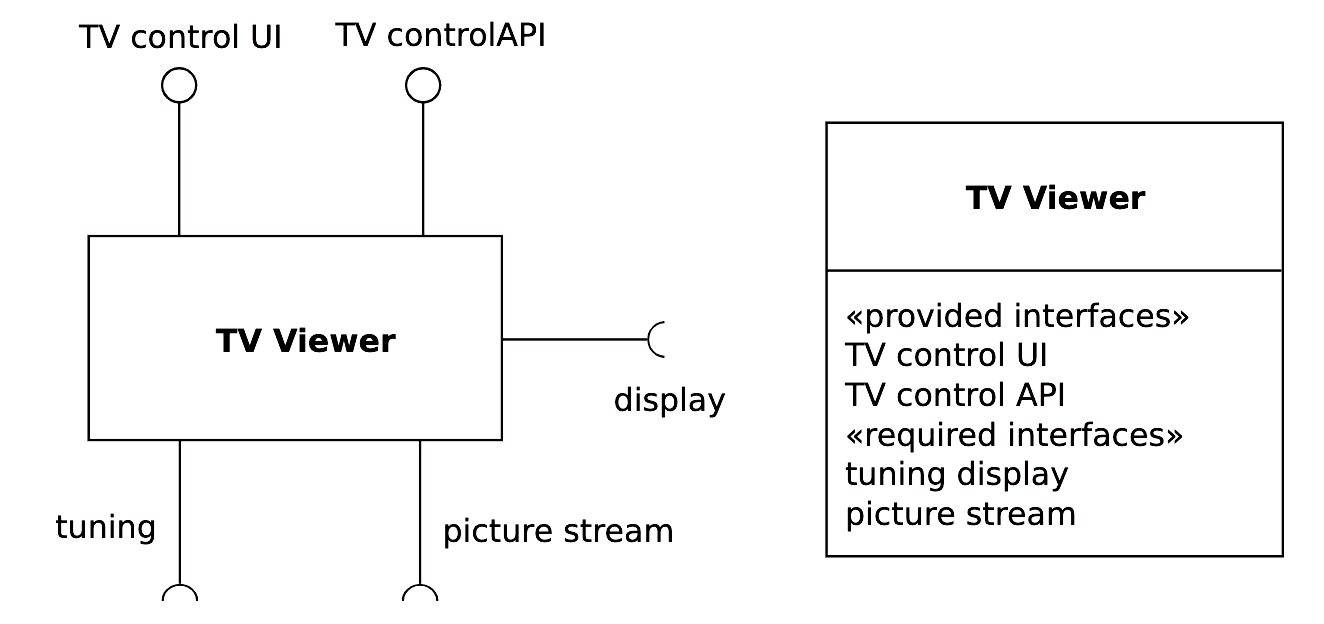
\includegraphics[width=0.75\linewidth]{assets/UML/struct_comp/struct_comp.png}
    \caption{Struttura interna della classe; le interfacce richieste/fornite sono raggruppate logicamente tramite "porte".}
\end{figure}

\paragraph{Esempio} TV Viewer: ogni istanza possiede un'istanza di TVPresenter e un'istanza di Generator (campi dell'oggetto), attraverso le quali fornisce e richiede determinate interfacce. Ogni proprietà posseduta dalla classe è una parte dell'istanza, indicata da \textbf{nome:classe} e dalla molteplicità. Le varie parti sono collegate da \textbf{connettori} (linee continue). I \textbf{connettori di delega} (frecce tratteggiate a punta aperta) collegano una parte alle interfacce che fornisce o richiede.

\begin{figure}[H]
    \centering
    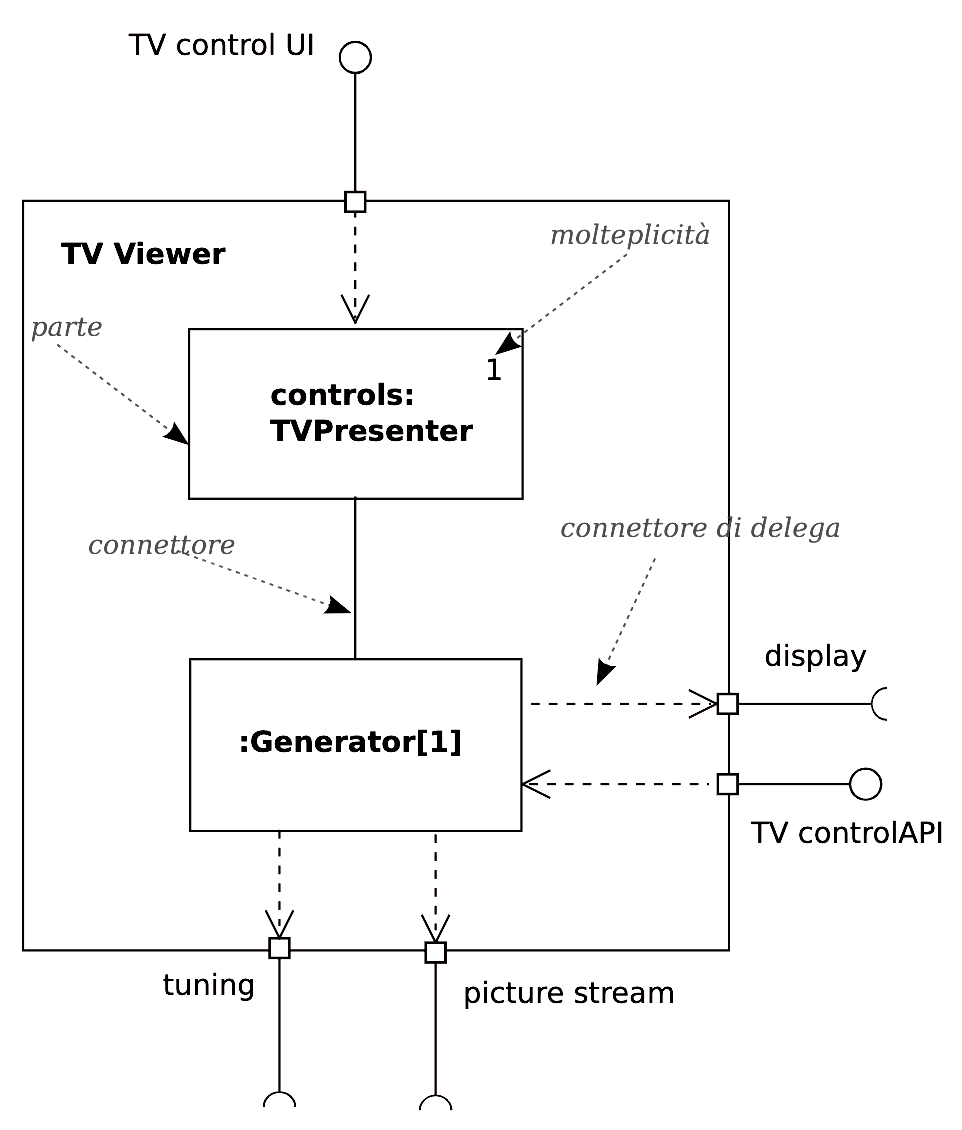
\includegraphics[width=0.4\linewidth]{assets/UML/struct_comp/struct_comp2.png}
    \caption{Esempio di structure composite (TV Viewer)}
\end{figure}

\newpage